% !TeX spellcheck = en_US

\chapter{Concept}
\label{chap:ch3}
The objective of this work is to evaluate the usefulness of an \gls{IDE} extension for the \gls{Gropius} system \cite{speth2020gropius}.
This chapter describes the approach taken in this thesis for archiving that goal.
At the heart of the concept is a plan to develop an issue management extension for one \gls{IDE},
which integrates into the  \gls{Gropius} framework.
This tool is then used in the evaluation by presenting to experts in the field for a review.

The first step was to gather requirements for that prototype. 
This requirements engineering process as well as its results are described in \cref{sec:ch3:s1}.
Visualizing details about an issue in the corresponding icon is a key part of multiple requirements.
Therefore, the next step was to determine which properties to visualize and how.
The resulting concept for the icons is explained in \cref{sec:ch3:s2}.
Finally, as described in \cref{sec:ch3:s3}, 
a rough concept for the extension was made before continuing with the design and implementation.

\section{Analysis and Requirements Engineering}
\label{sec:ch3:s1}
The goal of requirements engineering is to gather, document, validate and manage requirements for a computer-based system \cite{sommerville1997requirements}. 
To gather requirements for the extension, a process with six steps as shown in \cref{fig:requirmentsProcess} was used.
This process is split into two stages, each with the three activities of requirements elicitation, specification, and validation.

\begin{figure}[!h]
	\centering
	\tikzstyle{mybox} = [draw=blue!40, fill=blue!20, very thick,
	rectangle, rounded corners, inner sep=5pt, inner ysep=5pt,
	minimum width=0.45\linewidth, minimum height=80pt, text width=0.45\linewidth]
	\tikzstyle{title} = [fill=blue!40, rectangle, rounded corners]
	\begin{tikzpicture}
	\node[mybox] (box1) {
		\begin{varwidth}{\linewidth}\begin{itemize}
		\item Internal Brainstorming
		\end{itemize}\end{varwidth}
	};
	\node[title] (box1title) at (box1.north) {Requirements Elicitation};
	
	\node[mybox] (box2) [right=of box1] {
		\begin{varwidth}{\linewidth}\begin{itemize}
		\item Artifact: Thesis Proposal Paper
		\end{itemize}\end{varwidth}
	};
	\node[title] (box2title) at (box2.north) {Requirements Specification};
	
	\node[mybox] (box3) [below=of box2] {
		\vskip 0.3\baselineskip
		\begin{varwidth}{\linewidth}\begin{itemize}
		\item Thesis Proposal Paper Feedback
		\item Thesis Proposal Presentation Discussion and Feedback
		\end{itemize}\end{varwidth}
	};
	\node[title] (box3title) at (box3.north) {Requirements Validation};
	
	\node[mybox] (box4) [below=of box1] {
		\vskip 0.3\baselineskip
		\begin{varwidth}{\linewidth}\begin{itemize}
		\item Feedback from Thesis Propsal
		\item Internal Brainstorming
		\item Stakeholder Interview
		\end{itemize}\end{varwidth}
	};
	\node[title] (box4title) at (box4.north) {Requirements Elicitation};
	
	\node[mybox] (box5) [below=of box4] {
		\vskip 0.3\baselineskip
		\begin{varwidth}{\linewidth}\begin{itemize}
		\item Artifact: Requirements Document
		\end{itemize}\end{varwidth}
	};
	\node[title] (box5title) at (box5.north) {Requirements Specification};
	
	\node[mybox] (box6) [below=of box3] {
		\vskip 0.3\baselineskip
		\begin{varwidth}{\linewidth}\begin{itemize}
		\item Review through Supervisor
		\end{itemize}\end{varwidth}
	};
	\node[title] (box6title) at (box6.north) {Requirements Validation};
	
	\path [->,draw,thick] (box1) -- (box2);
	\path [->,draw,thick] (box2) -- (box3title);
	\path [->,draw,thick] (box3) -- (box4);
	\path [->,draw,thick] (box1) -- (box4title);
	\path [->,draw,thick] (box4) -- (box5title);
	\path [->,draw,thick] (box5) -- (box6);
	\end{tikzpicture}
	\caption{Requirements Engineering Process}
	\label{fig:requirmentsProcess}
\end{figure}

As the first step of the first stage, a preliminary requirements elicitation was performed. 
For this, internal brainstorming and discussion with the thesis' supervisors were used.
Next, the resulting requirements were incorporated into the proposal for this thesis, 
which serves as the first requirements specification.
After this, the primary requirements validation was performed. 
The positive feedback for that proposal paper was one of the signs that the requirements are valid.
Additionally, the discussion and feedback after the thesis proposal presentation was also used to validate the requirements.

Then, the second stage of requirements elicitation was performed using the requirements from the first elicitation, 
the results from the validation as well as the results of a stakeholder interview.
For this interview, the general concept of Gropius as well as of this thesis was sent to representatives of each group of stakeholders. 
They were then asked for their requirements with the help of two questions.
The first question asked for features expected from an issue management plugin in general,
the second for those, which the representatives would expect from such a plugin, which integrates into \gls{Gropius}.

Since the prototype is a new tool for a system under development, only three groups of stakeholders could be identified:
First, the potential users, in this case developers, working with component-based systems, such as microservices.
Various members of the department for software quality and architecture were contacted as representatives of this group.
Second, the thesis' supervisors to ensure the scientific scope of the work. 
Third, Sandro Speth, who is also one of the supervisors, as the author of the \gls{Gropius} system \cite{speth2020gropius}.

Next, the gathered requirements were formally specified as user stories in the requirements document.
Finally, this document was validated by a review from the thesis' supervisors.


\subsection*{Gathered Requirements}
The result of this requirements engineering process is a list of functional requirements in the form of user stories.
These requirements are listed below, split into those expected from any issue management plugin and those expected from a plugin integrated into \gls{Gropius}.

\newcounter{enumarteCounter} % For saving the counter between the two enumerates

First, the requirements expected from any issue management plugin:
\begin{enumerate}
	\item As a developer, I want to have a list of all open issues. \label{itm:ch3:req:filter_open}
	\item As a developer, I want to have a list of all issues assigned to me. \label{itm:ch3:req:filter_me}
	\item As a developer, I want to have a searchable list of issues. \label{itm:ch3:req:filter_search}
	\item As a developer, I want to have a list of issues that can be filtered by tags or labels. \label{itm:ch3:req:filter_labels}
	\item As a developer, I want to have a list of issues which can be filtered to only show issues relevant to my currently opened project. \label{itm:ch3:req:filter_open project}
	\item As a developer, I want to have a list of issues which can be filtered to only show issues relevant to my currently opened source file. \label{itm:ch3:req:filter_open_file}
	\item As a developer, I want to quickly see the type of an issue in this list. \label{itm:ch3:req:list_issue_type}
	\item As a developer, I want to be able to see all details for a specific issue.
	\item As a developer, I want to be able to jump to a related issue from my currently viewed issue.
	\item As a developer, I want to be able to quickly open a relevant source file at the relevant line for an issue, even if it is in another eclipse project (as long as that project is in my workspace).
	\item As a developer, I want to be shown which lines of a source file are relevant for an issue. (For example through markers at the side of the editor) \label{itm:ch3:req:source_file_marker}
	\item As a developer, I want to be able to edit every property of an issue that I have write access to.
	\item As a developer, I want to be able to create a new issue.
	\item As a developer, I want to be able to create a new issue for some lines of code without manually entering the source file and lines in a dialog.
	\setcounter{enumarteCounter}{\value{enumi}} % store counter to continue later
\end{enumerate}

These are the requirements expected from such a plugin integrated into \gls{Gropius}:
\begin{enumerate}
	\setcounter{enumi}{\value{enumarteCounter}} % restore counter from above
	\item As a developer, I want the system architecture graph in my web browser to focus on the component I've selected in eclipse.
	\item As a developer, I want the system architecture graph in my web browser to highlight the issue I've selected in eclipse.
	\item As a developer, I want to be able to open details about an issue in the eclipse view through the architecture graph in my web browser.
	\item As a developer, I want to be able to open a relevant source code line of an issue in eclipse from the architecture graph in my web browser.
	\item As a developer, I want to be able to have the possibility to set the focus of the architecture graph and eclipse editor as well as the issue view of my colleagues, for example in meetings.
\end{enumerate}

\section{Concept for the Issue Icons}
\label{sec:ch3:s2}
For requirements \ref{itm:ch3:req:list_issue_type} and \ref{itm:ch3:req:source_file_marker}, it is useful to have icons for each issue.
Especially for requirement \ref{itm:ch3:req:list_issue_type} the icons can not all be the same but need to carry some information.
Therefore, a concept was made about which properties should be visualized in these icons.

One possible property is the type of issue.
As described in \cref{ssec:ch2:ss1.1} an issue can represent various concepts.
The type of issue can be used to roughly specify which of these concepts is represented by an issue.
Common values are bug and enhancement.

Another interesting concept, that could be visualized in the icons, is the idea that one issue can be the cause of another.
For example a Null-Pointer in one component could cause an illegal response in an \gls{API}, which could cause a crash in another component.
Then the Null-Pointer is the root cause.
The illegal response is a symptom of that but also the cause of the crash.
The crash is just a symptom of the illegal response and can probably not be completely fixed without fixing the other two.

Other interesting properties include, to whom the issue is assigned and the state of the issue.
It could be interesting to immediately recognize issues assigned to yourself.
With the state of the issue a developer can directly see if the issue still exists and if work is required.

As it was not clear how much information could be visualized in one small icon, 
the properties that should be visualized were ordered by their priority.
That way it was easier to make decisions about what information to include in the icon and how prominent to visualize it later during the creation of these icons.
The following properties were chosen to be visualized with decreasing priority.
\begin{itemize}
	\item Type of Issue
	\subitem Enhancement vs. Bug
	\item Does this issue cause problems in other projects/components?
	\item Is this issue just a symptom of another issue elsewhere or is this the root cause?
	\item Is the issue assigned to the viewing developer?
	\item Is the issue new or work in progress or done?
\end{itemize}
Finally, another aspect, that could be visualized is the visibility of the issue as some \glspl{IMS} can have issues that are only visible internally.
However, it was decided against it for now, as it didn't seem that important of a property and the Gropius system currently doesn't support it anyway.

\section{Concept for the Prototype Plugin}
\label{sec:ch3:s3}
Before starting with the detailed design and implementation of the prototype tool, a rough concept for it needed to be created.
Most parts of this were already done during the thesis' proposal process and a version of this concept was included in the proposal paper.
Therefore, the feedback for the paper and the presentation in front of the department was a confirmation, that the general concept is reasonable.

According to the concept, the plugin consists of two main \gls{UI} elements: The issue list and the issue details element.
These are complemented by various dialogs and other features described below.
The plugin uses the \gls{API} of the \gls{Gropius} system to retrieve the required data and perform any modifications on it.
Furthermore, the plugin is split into multiple components, 
of which only one is specific to the supported \gls{IDE} 
and the others are reusable for other \glspl{IDE} with minimal changes.
That way the amount of work to port it for another \gls{IDE} is minimized,
as long as it supports \gls{java}-based plugins.

\begin{figure}[!h]
	\centering
	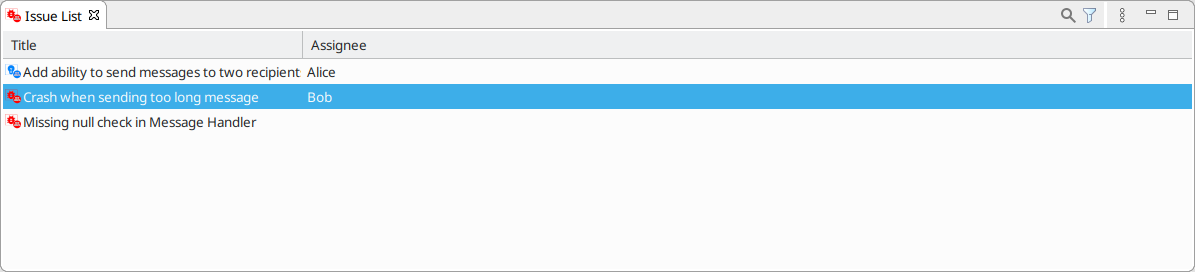
\includegraphics[width=\textwidth]{graphics/concept_mockup_issueList.png}
	\caption{Mock-up for Issue List}
	\label{fig:c3:mockup_issueList}
\end{figure}
The issue list is a table of issues with columns for the various properties of those, 
similar to the one shown in the mock-up in \cref{fig:c3:mockup_issueList}.
In the first column, the icon for the issue is shown followed by the title.
This table allows filtering by various attributes of the issues.
To satisfy requirements \ref{itm:ch3:req:filter_open} to \ref{itm:ch3:req:filter_open_file} it supports at least filtering
by issue state, assignee, text contained in the title or description, 
labels as well as whether the issue is relevant to the open \gls{IDE} project or the open file.
Furthermore, it is possible to sort the table based on any column. 
Finally, the visible columns can also be configured by the user.

\begin{figure}[!h]
	\centering
	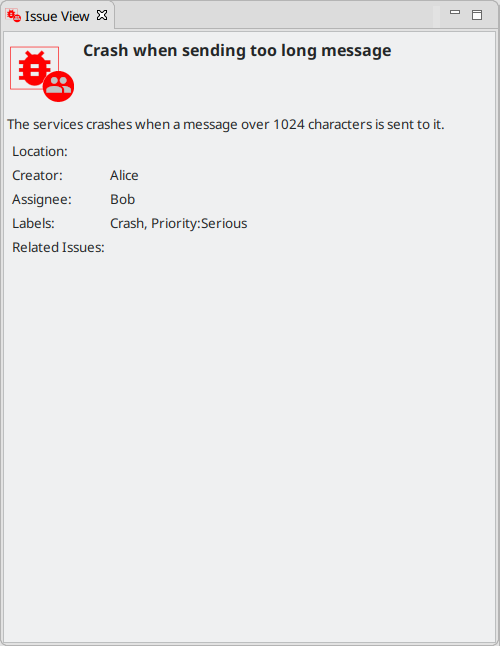
\includegraphics[width=0.5\textwidth]{graphics/concept_mockup_issueDetails.png}
	\caption{Mock-up for Issue Details}
	\label{fig:c3:mockup_issueDetails}
\end{figure}
The issue details \gls{UI} element shows all attributes for the issue selected in the issue list.
A mock-up of it can be seen in \cref{fig:c3:mockup_issueDetails}.
At the top of the form, the icon of the issue is displayed.
The related issues are links, which, when clicked, change the issue list selection to the corresponding issue.
Furthermore, the displayed locations are also links, which open the correct resource in the \gls{IDE}'s editor.
Additionally, this element supports editing the issue, either by opening a dialog or by allowing to edit the values in the element itself like a form.
In both cases, additional dialogs are used to allow editing of the more complex attributes. 

\begin{figure}[!h]
	\centering
	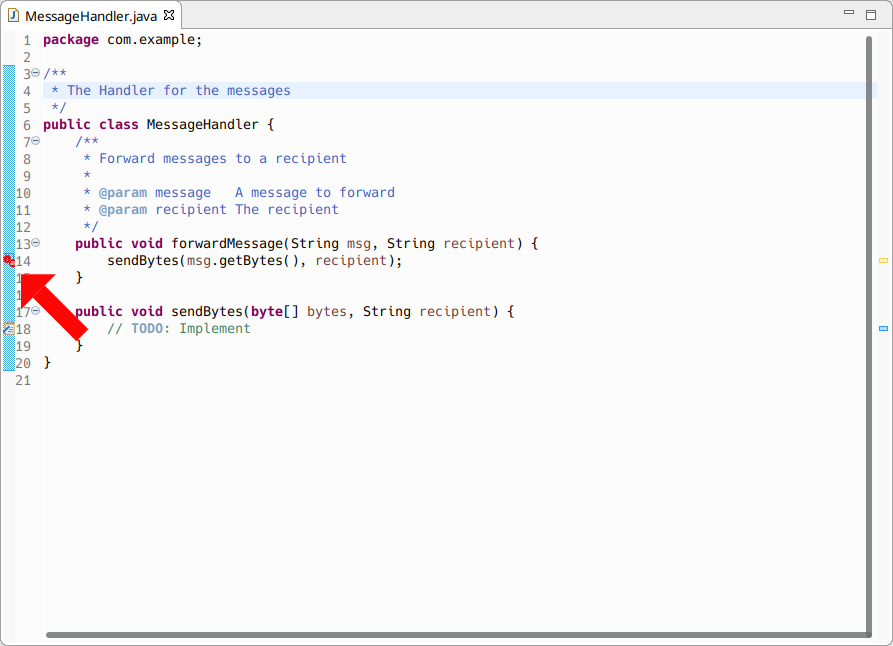
\includegraphics[width=0.75\textwidth]{graphics/concept_mockup_issueMarker_arrow.png}
	\caption{Mock-up of Issue in the Marker Column}
	\label{fig:c3:mockup_issueMarkers}
\end{figure}
Moreover, the issues are displayed as markers in the \gls{IDE}'s editor, whenever a file with issues is open in the editor.
This can be seen in the mock-up in \cref{fig:c3:mockup_issueMarkers}. 
For these the icons from \cref{sec:ch3:s2} are used, if the \gls{IDE} supports it.

Additionally, there are two ways to create a new issue.
First, there is a button somewhere, which creates a new empty issue, 
optionally opening a dialog to enter details for the new issue.
Second, it is possible to mark some lines in the editor and create a new issue for them.
In this case, the new issue already has the correct location selected.

\begin{figure}[!h]
	\centering
	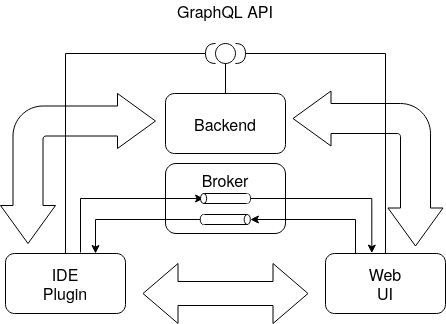
\includegraphics[width=0.5\textwidth]{graphics/concept_gropius_frontend_messaging.png}
	\caption{Messaging Concept for Gropius Frontend Integration}
	\label{fig:c3:concept_gropius_messaging}
\end{figure}

Finally, the tool is connected to the existing web \gls{UI} with the help of a messaging component.
That way it is possible to enable synchronization between the plugin and the web user interface, 
such that selecting an issue in one will cause the other to also jump to the same issue and select it accordingly. 
Each user has a separate topic in the messaging component, preventing undesirable interaction between multiple users. 
In addition to this, special topics for example for meetings are a possibility, 
such that one developer can select an issue and the same is selected for all other participants of the meeting. 
\cref{fig:c3:concept_gropius_messaging} shows the basic architecture planned for this feature. 
The plugin, as well as the web user interface, communicate with the back-end through a \gls{REST} \gls{API} and with each other using a messaging component.
